\documentclass[a4paper,12pt]{article}
\usepackage[left=2.5cm, right=2.5cm, top=2.5cm, bottom=2.5cm]{geometry}
\usepackage{amssymb}
\usepackage[backend=biber]{biblatex}
\addbibresource{../bibliography.bib}
\usepackage{minted}
\setminted{frame=lines, fontsize=\small}
\usepackage{graphicx}
\usepackage{hyperref}
\hypersetup{
    colorlinks=true,
    linkcolor=black,
    filecolor=black,
    urlcolor=black,
    citecolor=black
}
% Allow more flexible breaking of long URLs:
\setlength\emergencystretch{3em}
\setcounter{biburllcpenalty}{7000}
\setcounter{biburlucpenalty}{7000}
\Urlmuskip=0mu plus 1mu

\title{Distance-based dimensionality reduction for big data literature review}
\author{Adrià Casanova Lloveras}

\begin{document}

\maketitle

\tableofcontents
\pagebreak

\section{\texttt{Rdimtools}: An R Package for Dimension Reduction
and Intrinsic Dimension Estimation \texorpdfstring{\cite{Rdimtools}}{}}
\label{sec:rdimtools}


\subsection{Abstract}

\paragraph{Original:} Discovering patterns of the complex high-dimensional data is one of the fundamental pillars of modern data science. Dimension reduction and intrinsic dimension estimation are two thematic programs that facilitate geometric characterization of the data. We present \texttt{Rdimtools}, an R package that supports 143 dimension reduction and manifold learning methods and 17 dimension estimation algorithms whose unprecedented extent makes multifaceted scrutiny of the data in one place easier. \texttt{Rdimtools} is distributed under the MIT license and is accessible from CRAN, GitHub, and its package website, all of which deliver instruction for installation, self-contained examples, and API documentation.

\paragraph{Apple Intelligence summary:} \texttt{Rdimtools}, an R package, supports 160 dimension reduction and manifold learning methods, making data analysis easier. It is available on CRAN, GitHub, and its package website.

\subsection{Key Points}

\begin{itemize}
    \item \textbf{R package}: that supports 143 dimension reduction and manifold learning methods and 17 dimension estimation algorithms.
    \item \textbf{Other libraries}: \texttt{drtoolbox} in MATLAB, \texttt{scikit-learn} in Python, a C++ template library \texttt{tapkee} with a known basis of popularity. In R, packages \texttt{dimRed}, \texttt{dyndimred}, \texttt{intrinsicDimension}.
    \item \textbf{Implementation}: mixture of R and C++ that are integrated by \texttt{Rcpp}. For numerical operations, \texttt{RcppArmadillo} is heavily used to take advantage of \texttt{Armadillo} C++ linear algebra library.
    \item  \textbf{3 function families}: \verb|do.{algorithm}|, \verb|est.{algorithm}| and \verb|aux.{algorithm}| for DR, IDE, and auxiliary functions.
    \item Downloaded 1013 times per month on average from CRAN.
    \item \textbf{Future plan}: support for out-of-memory execution in response to the increased needs for big data analysis.
\end{itemize}

\subsection{Example R Code}

\begin{minted}{r}
    # Documentation example:
    # do.idmap (Interactive Document Map)

    library(Rdimtools)

    ## load iris data
    data(iris)
    set.seed(100)
    subid = sample(1:150,50)
    X = as.matrix(iris[subid,1:4])
    lab = as.factor(iris[subid,5])
    ## let's compare with other methods
    out1 <- do.pca(X, ndim=2)
    out2 <- do.lda(X, ndim=2, label=lab)
    out3 <- do.idmap(X, ndim=2, engine="NNP")
    ## visualize
    opar <- par(no.readonly=TRUE)
    par(mfrow=c(1,3))
    plot(out1$Y, pch=19, col=lab, main="PCA")
    plot(out2$Y, pch=19, col=lab, main="LDA")
    plot(out3$Y, pch=19, col=lab, main="IDMAP")
    par(opar)
\end{minted}

\begin{figure}[ht]
    \centering
    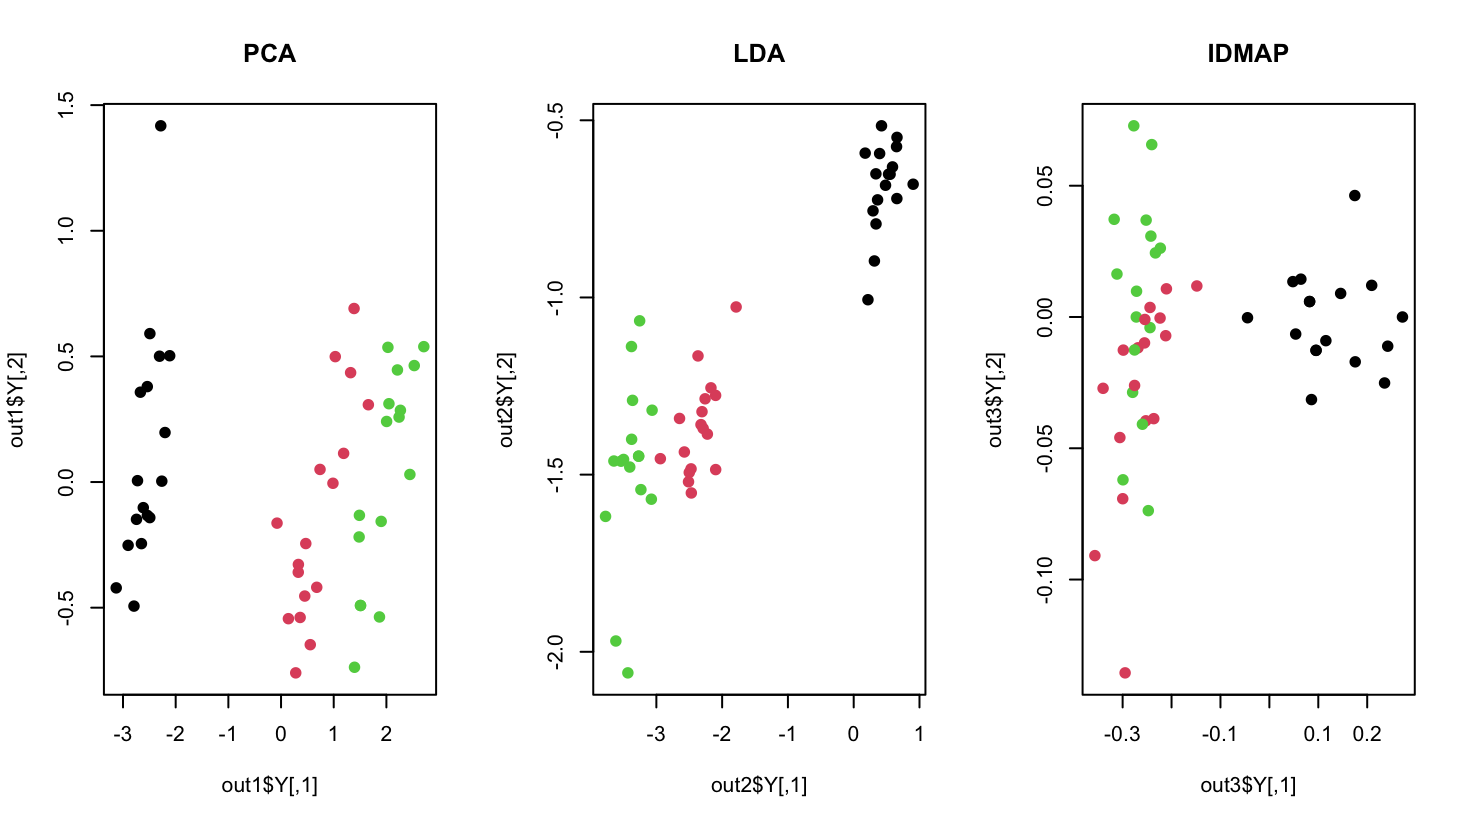
\includegraphics[width=0.8\textwidth]{figures/Rdimtools_test.png}
    \caption{Rdimtools test output.}
    \label{fig:rdimtools_test}
\end{figure}

\pagebreak
\section{Global versus local methods in nonlinear dimensionality reduction \texorpdfstring{\cite{deSilvaTenenbaum2002}}{}}
\label{sec:deSilvaTenenbaum2002}

\subsection{Abstract}

\paragraph{Original:} Recently proposed algorithms for nonlinear dimensionality reduction fall broadly into two categories which have different advantages and disadvantages: global (Isomap), and local (Locally Linear Embedding, Laplacian Eigenmaps). We present two variants of Isomap which combine the advantages of the global approach with what have previously been exclusive advantages of local methods: computational sparsity and the ability to invert conformal maps.

\paragraph{Apple Intelligence summary:} Two new Isomap variants are presented, combining global advantages with local computational sparsity and conformal map inversion.

\subsection{Key Points}

\begin{itemize}
    \item \textbf{Introduction of LMDS} by applying it to Isomap (L-Isomap).
    \item \textbf{\textit{Landmark points}} $(n << N)$ reduce the complexity of computing:
    \begin{itemize}
        \item the distances matrix with Dijkstra's algorithm with Fibonacci heaps ($k$ = neighborhood size) from $\mathcal{O}(kN^2\log N)$ to $\mathcal{O}(knN\log N)$.
        \item MDS from $\mathcal{O}(n^3)$ to $\mathcal{O}(n^2N)$.
    \end{itemize}
    \item If $x$ is a landmark point, then the embedding given by LMDS is consistent with the original MDS embedding.
    \item If the distance matrix $D_{n,N}$ can be represented exactly by a Euclidean configuration in $\mathbb{R}^l$, and if the landmarks are chosen so that their affine span in that the configuration is $l$-dimensional (i.e. general position), then LMDS will recover the configuration exactly, up to rotation and translation.
\end{itemize}

\begin{figure}[ht]
    \centering
    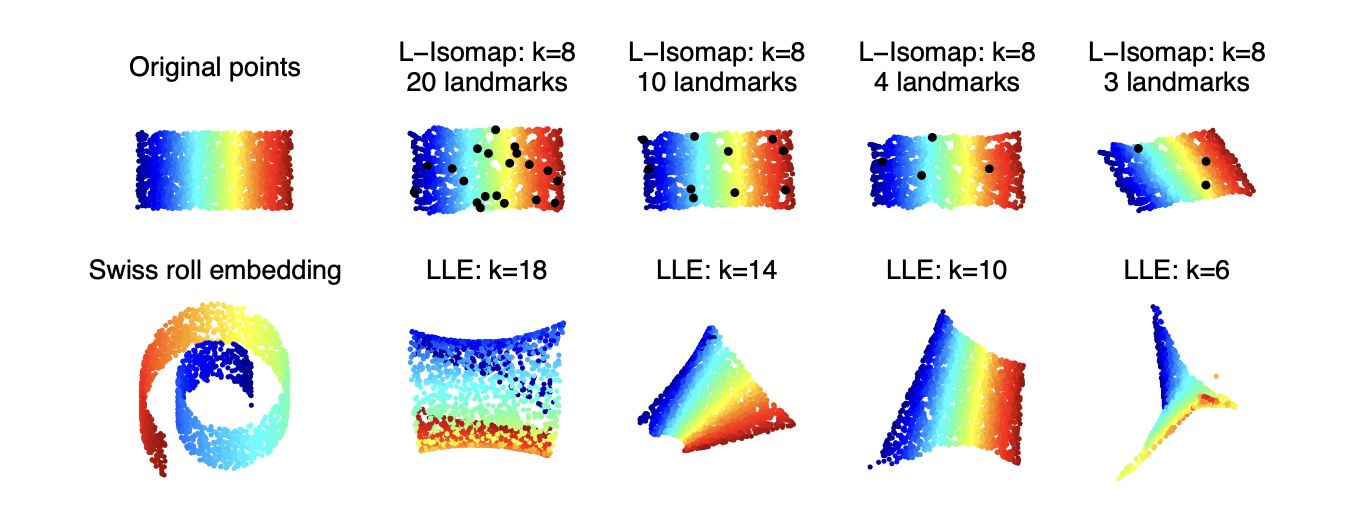
\includegraphics[width=0.8\textwidth]{figures/LMDS_3.png}
    \caption{L-Isomap is stable over a wide range of values for the sparseness parameter (the number of landmarks). Results from LLE are shown for comparision\cite{deSilvaTenenbaum2002}.}
    \label{fig:LMDS}
\end{figure}


\pagebreak
\section{\texttt{dimRed} and \texttt{coRanking} - Unifying Dimensionality Reduction in R \texorpdfstring{\cite{Kraemer2018dimRedAC}}{}}
\label{sec:Kraemer2018dimRedAC}

\subsection{Abstract}

\paragraph{Original:} “Dimensionality reduction” (DR) is a widely used approach to find low dimensional and interpretable representations of data that are natively embedded in high-dimensional spaces. DR can be realized by a plethora of methods with different properties, objectives, and, hence, (dis)advantages. The resulting low-dimensional data embeddings are often difficult to compare with objective criteria. Here, we introduce the \texttt{dimRed} and \texttt{coRanking} packages for the R language. These open source software packages enable users to easily access multiple classical and advanced DR methods using a common interface. The packages also provide quality indicators for the embeddings and easy visualization of high dimensional data. The \texttt{coRanking} package provides the functionality for assessing DR methods in the co-ranking matrix framework. In tandem, these packages allow for uncovering complex structures high dimensional data. Currently 15 DR methods are available in the package, some of which were not previously available to R users. Here, we outline the \texttt{dimRed} and \texttt{coRanking} packages and make the implemented methods understandable to the interested reader.

\paragraph{Apple Intelligence summary:} Dimensionality reduction (DR) methods create low dimensional data representations, but comparison is challenging. The \texttt{dimRed} (figure \ref{fig:dimRed_methods}) and \texttt{coRanking} R packages are introduced to address this.

\subsection{Key Points}

\begin{itemize}
    \item The difficulty in applying DR is that each DR method is designed to maintain certain aspects of the original data and therefore may be appropriate for one task and inappropriate for another. Most methods also have parameters to tune and follow different assumptions.
    \item \textbf{Software packages for other languages}:
        \begin{itemize}
            \item Python: \texttt{scikit-learn}, which contains a module for DR.
            \item Julia: \texttt{ManifoldLearning.jl} for nonlinear and \texttt{MultivariateStats.jl} for linear DR.
            \item Matlab: several toolboxes.
            \item C++: \texttt{Shogun} toolbox, which offers bindings for many high level languages (including R).
        \end{itemize}
    \item At the time (2018), no comprehensive package for R.
    \item None of the former provides means to consistently compare the quality of different methods.
    \item MDS can be seen as kPCA with kernel $x^T y$, since a distance matrix can be transformed to a matrix of inner products.
    \item \texttt{dimRed} wraps \texttt{cmdscale}.
    \item In contrast to a supervised problem, there is no natural way to directly measure the quality of any output or to compare two methods. Every
    method optimizes a different error function.
    \item \textbf{Quality criteria implemented in \texttt{coRanking}}:
        \begin{itemize}
            \item \textbf{Co-ranking matrix based measures}: the co-ranking matrix $Q$ is the 2d-histogram of the distance ranks. $q_{ij}$ is an integer which counts how many points of distance rank $j$ became rank $i$. In a perfect DR, this matrix will only have non-zero entries in the
            diagonal. In R, the co-ranking matrix can be calculated using the the \texttt{coRanking::coranking} function. The \texttt{dimRed} package contains the functions \texttt{Q\_local, Q\_global, Q\_NX, LCMC}, and \texttt{R\_NX} to calculate the above quality measures in addition to \texttt{AUC\_lnK\_R\_NX}. If $R_{NX}$ is high for low values of $K$, then local neighborhoods are maintained well; if $R_{NX}$ is high for large values of $K$, then global gradients are maintained well (see fig. \ref{fig:dimRed_R_NX}).
            \item Cophenetic correlation.
            \item \textbf{Reconstruction error}: the fairest one when the method provides an inverse mapping. $\mathrm{RMSE}=\sqrt{\frac{1}{n} \sum_{i=1}^n d\left(x_i^{\prime}, x_i\right)^2}$, with $x_i' = f^{-1}(y_i) = f^{-1}(f(x_i))$.
        \end{itemize}
    \item \textbf{Test datasets}: Common ones being the 3d S-curve and the Swiss roll. Real world examples usually have more dimensions and often are much noisier and we cannot be sure if we can observe all the relevant variables. Can be retrieved with \texttt{dimRed::loadDataSet}
    \item \textbf{Main functions:} \texttt{embed, quality, plot, plot\_R\_NX}.
\end{itemize}

\begin{figure}[ht]
    \centering
    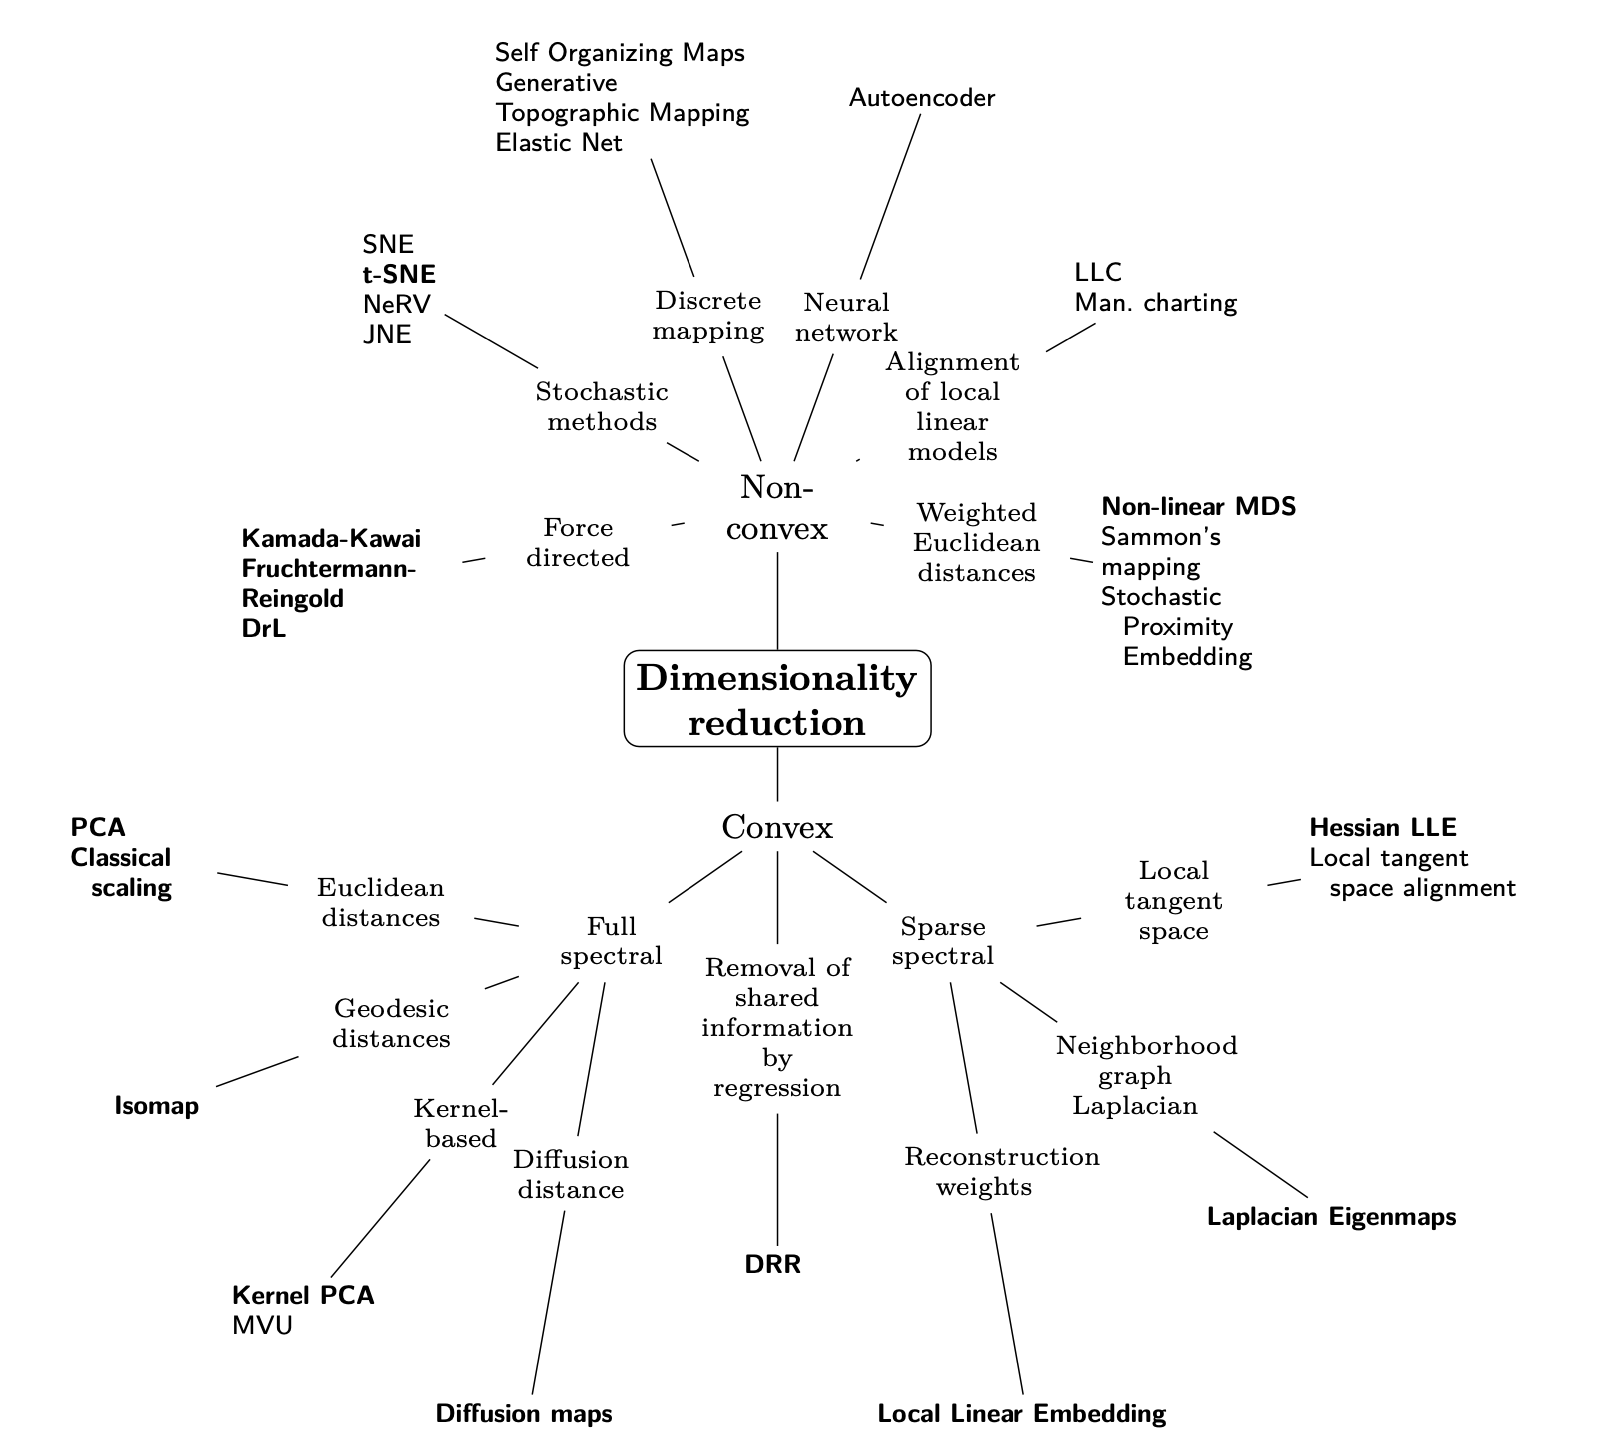
\includegraphics[width=0.8\textwidth]{figures/dimRed_methods.png}
    \caption{DR methods implemented in \texttt{dimRed} \cite{Kraemer2018dimRedAC}.}
    \label{fig:dimRed_methods}
\end{figure}

\begin{figure}[ht]
    \centering
    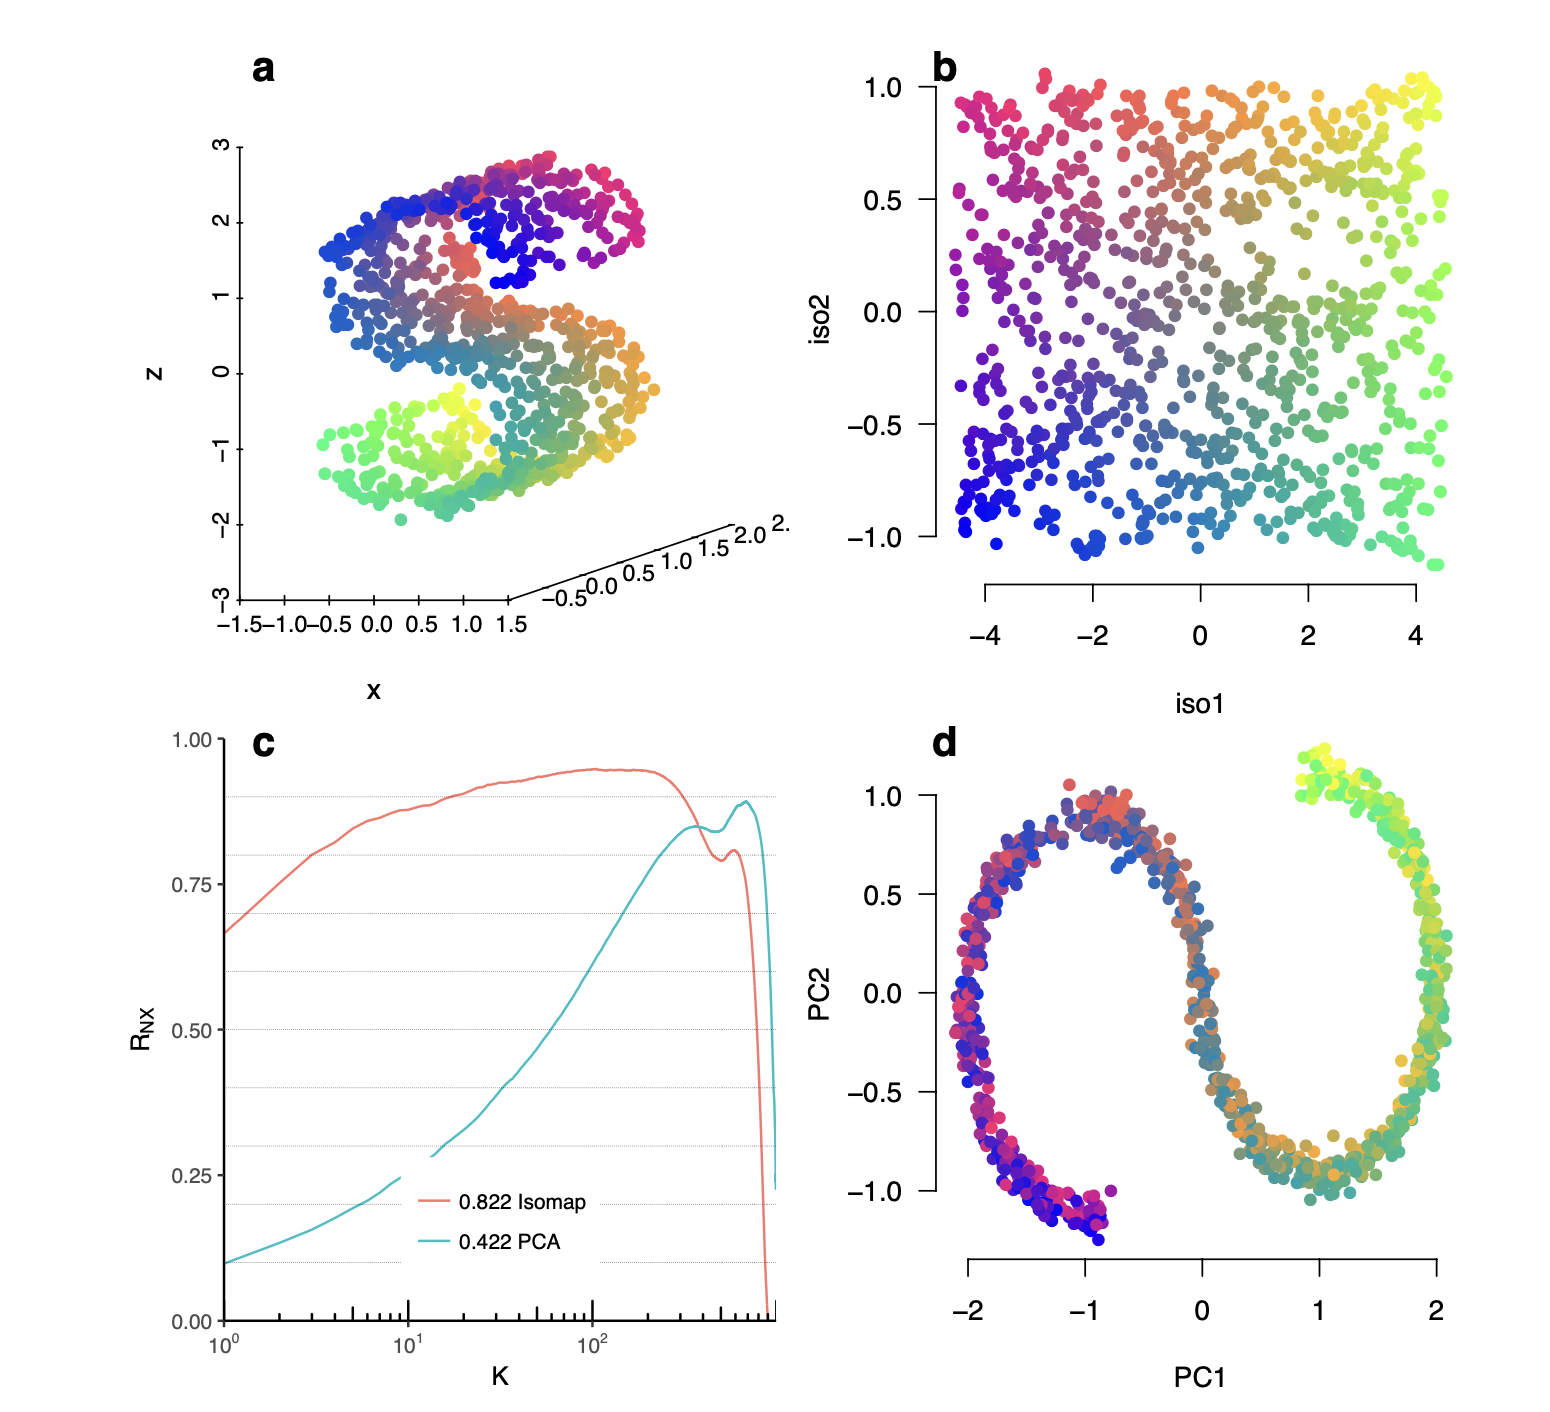
\includegraphics[width=0.8\textwidth]{figures/dimRed_R_NX.png}
    \caption{$R_{NX}$ measures the quality of the embedding. \cite{Kraemer2018dimRedAC}.}
    \label{fig:dimRed_R_NX}
\end{figure}


\pagebreak
\section{Sparse multidimensional scaling
using landmark points \texorpdfstring{\cite{LMDS:2004}}{}}
\label{sec:LMDS:2004}

\subsection{Abstract}

\paragraph{Original:} In this paper, we discuss a computationally efficient approximation to the classical multidimensional scaling (MDS) algorithm, called Landmark MDS (LMDS), for use when the number of data points is very large. The first step of the algorithm is to run classical MDS to embed a chosen subset of the data, referred to as the 'landmark points', in a low-dimensional space. Each remaining data point can be located within this space given knowledge of its distances to the landmark points. We give an elementary and explicit theoretical analysis of this procedure, and demonstrate with examples that LMDS is effective in practical use.

\paragraph{Apple Intelligence summary:} Landmark MDS approximates classical multidimensional scaling for large datasets. It embeds a subset of data points, called “landmark points”, in a low-dimensional space, then locates remaining points based on their distances to these landmarks.


\subsection{Key Points}

\begin{itemize}
    \item \textbf{LMDS}: Landmark MDS.
    \item \textbf{Method}:
        \begin{enumerate}
            \item Select $n$ landmark points from $N$ data points.
            \item Apply MDS to the $n \times n$ distance matrix to obrain $L$.
            \item Embed remaining points via distance-based triangulation.
        \end{enumerate}
    \item \textbf{Complexity}: Classical MDS: $\mathcal{O}(N^2)$ storage, $\mathcal{O}(N^3)$ time. LMDS: $\mathcal{O}(nN)$ storage, lower time complexity.
    \item It has links with Isomap (L-Isomap), the Nyström method (which finds approximate solutions to a positive semi-definite symmetric eigenvalue problem using just a few of the columns of the matrix) and FastMap.
\end{itemize}


\pagebreak
\section{Comparative study for dimensionality reduction techniques for big data \texorpdfstring{\cite{SalahHenouda2020}}{}}
\label{sec:SalahHenouda2020}

\subsection{Abstract}

\paragraph{Original:} Nowadays, big data represents the solution for different type of users especially enterprises due to its huge amount of information augmented in real time. All these generated data could be described in one of big data characteristics named variety. One of the most challenging issues
for big data variety is high dimensionality because, it prevents the analysis process, demands heavy computations and adds noise to our data. The solution for this challenging issue is dimensionality reduction which minimize the dimensions and keeps only the essential information that give accurate results during analysis and decrease the computations complexity.

This paper aims to summarise and compare some of the recent methods that are used to solve the problem of high dimensionality in big data, Thereby, facilitating the process of research in this field.

\paragraph{Apple Intelligence summary:} High dimensionality in big data poses challenges, requiring dimensionality reduction to minimize dimensions and retain essential information. This paper compares recent methods for solving this problem, aiding research in the field.


\subsection{Key Points}

\begin{itemize}
    \item \textbf{Techniques Compared:}
        \begin{itemize}
            \item Classical/Modified PCA (modified to handle memory limits via row-scanning and MapReduce).
            \item Simplicial Nonnegative Matrix Tri-Factorization (SNMTF), an improved variant of NMF.
            \item Stacked Autoencoders, which yield lower reconstruction error than PCA.
            \item Linguistic Hedges Neuro-Fuzzy Classifiers with Feature Selection (LHNFCSF), a combination of neural networks and fuzzy inference systems (neuro-fuzzy) based on linguistic hedges with feature selection method.
            \item Deep Belief Networks (DBNs), which consist of multiple hidden layers where each layer is an RBM (Restricted Boltzman Machine), which is also a class of neural networks. Each RBM is connected with two layers, a hidden layer and a visible layer, and so on.
        \end{itemize}
\end{itemize}


\pagebreak
\section{Out-of-Core Dimensionality Reduction for Large Data via Out-of-Sample Extensions \texorpdfstring{\cite{reichmann2024outofcoredimensionalityreductionlarge}}{}}
\label{sec:reichmann2024outofcoredimensionalityreductionlarge}

\subsection{Abstract}

\paragraph{Original:} Dimensionality reduction (DR) is a well-established approach for the visualization of high-dimensional data sets. While DR methods
are often applied to typical DR benchmark data sets in the literature, they might suffer from high runtime complexity and memory requirements, making them unsuitable for large data visualization especially in environments outside of high-performance computing. To perform DR on large data sets, we propose the use of out-of-sample extensions. Such extensions allow inserting new data into
existing projections, which we leverage to iteratively project data into a reference projection that consists only of a small manageable subset. This process makes it possible to perform DR out-of-core on large data, which would otherwise not be possible due to memory and runtime limitations. For metric multidimensional scaling (MDS), we contribute an implementation with out-of-sample projection capability since typical software libraries do not support it.

We provide an evaluation of the projection quality of five common DR algorithms (MDS, PCA, t-SNE, UMAP, and autoencoders) using quality metrics from the literature and analyze the trade-off between the size of the reference set and projection quality. The run-time behavior of the algorithms is also quantified with respect to reference set size, out-of-sample batch size, and dimensionality of the data sets. Furthermore, we compare the out-of-sample approach to other recently introduced DR methods, such as PaCMAP and
TriMAP, which claim to handle larger data sets than traditional approaches. To showcase the usefulness of DR on this large scale, we contribute a use case where we analyze ensembles of streamlines amounting to one billion projected instances.

\paragraph{Apple Intelligence summary:} The study compares out-of-sample DR methods with PaCMAP and TriMAP on large datasets.  A use case demonstrates the usefulness of DR on a dataset of one billion projected streamline instances.

\subsection{Key Points}

\begin{itemize}
    \item A framework for OOS extensions of DR methods similar to Interpolation MDS.
    \item Applied to PCA, MDS, t-SNE, UMAP and autoencoders.
    \item Compared to TriMap and PaCMAC, which are efficient DR methods suitable for big data.
\end{itemize}

\begin{figure}[ht]
    \centering
    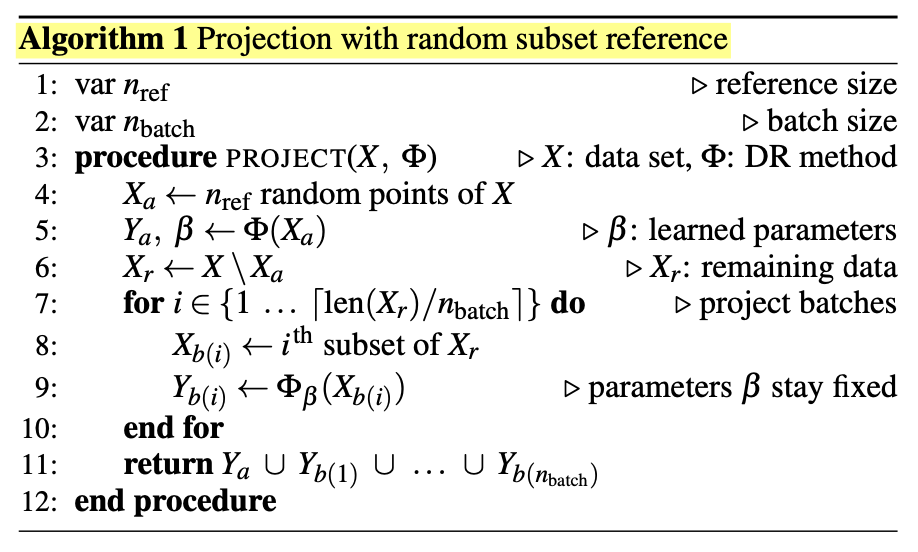
\includegraphics[width=0.8\textwidth]{figures/OOS_algorithm.png}
    \caption{OOS algorithm \cite{reichmann2024outofcoredimensionalityreductionlarge}.}
    \label{fig:OOS_algorithm}
\end{figure}

\begin{figure}[ht]
    \centering
    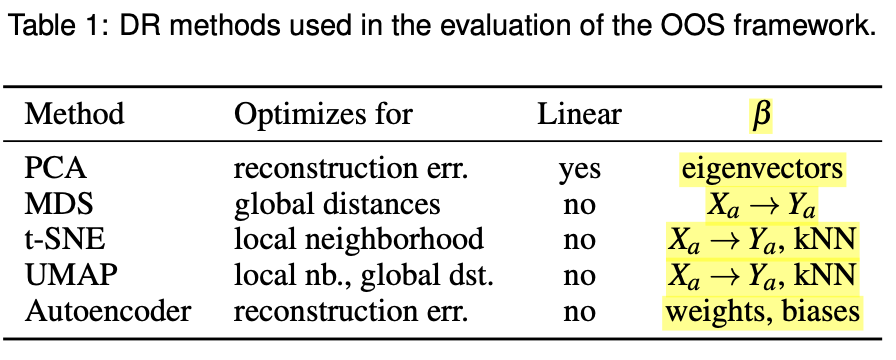
\includegraphics[width=0.8\textwidth]{figures/OOS_methods.png}
    \caption{OOS methods \cite{reichmann2024outofcoredimensionalityreductionlarge}.}
    \label{fig:OOS_methods}
\end{figure}


\pagebreak
\section{Title \texorpdfstring{TEXstring}{}}
\label{sec:}

\subsection{Abstract}

\paragraph{Original:}

\paragraph{Apple Intelligence summary:}


\subsection{Key Points}

\begin{itemize}
    \item 
\end{itemize}


\pagebreak
\printbibliography

\end{document}